\section{Methods}
% Here we describe the system used in this paper and detail the experiments conducted. 

\subsection{Evolution system}
% We used a minimal agent-based digital evolution model where each organism consists of a single integer genome, where fitness is determined as the expinentiation of the result of a sawtooth function based on genome value ($x$).
% To calculate fitness we first generate a score using a ``sawtooth'' function, similar to the one used by [CITE preprint], to create a landscape where local optima are separated by deleterious valleys.  
% Our sawtooth function (\(s\)) is defined as follows: 
% \[
% s(x) = kx - (k+d)(x\ \text{mod}\ w)
% \]
In order to isolate the adaptive momentum effect and keep computational costs feasible, we used a minimal agent-based evolution model where each organism's genome consists of a single integer, with value $x$. 
Fitness is based in a repeated ``sawtooth'' function, similar to the one used in \citep{Bohm2024.04.08.588357}, to create a landscape with regular fitness peaks separated by valleys. 
Each organism is assigned a quality score ($s(x)$), and then that score exponentiated to determine fitness ($f(x)=10^{s(x)}$). 
Score is calculated using the sawtooth function:

% \[
% s(x) = \frac{g}{w}x - (\frac{g}{w}+d)(x\ \text{mod}\ w)
% \]
\[
s(x) = \frac{x - (x~\text{mod}~w)}{w}G - (x~\text{mod}~w)D
\]

\noindent
where $G$ is the gain per peak, $D$ is the decrease per step into the valley, and $w$ is the valley width (number of mutational steps from one peak to the next). 
Effectively, the score function calculates the quality of the highest peak achieved and subtracts the cost of the current mutational step into the valley. 
%We used values of \(k = \frac{1}{6}\), \(a = w = 6\), and \(d = 0.05\).
We used $G=1.0$, $D=0.05$, and $w=6$.
This means that peaks appear every six steps; in this case at $x=6$, $x=12$, $x=18$, and so forth.
We refer to these peaks by their height, so those three peaks would be \(p_{1}\), \(p_{2}\), and \(p_{3}\), respectively.
We refer to the steps between peaks by the prior peak and an offset (\textit{e.g.}, $x=17$ is $p_{2} + 5$, the last step before $p_{3}$).
Figure \ref{fig-sawtooth} illustrates this sawtooth function and the relevant peaks.

Crossing a valley increases an organism's fitness by a factor of 10, and each step into the valley reduces fitness by \localapprox 12\%, relative to the previous peak. %regardless of which peak the organism was on.
We selected these drastic fitness differences to clearly demonstrate the effect.% rather than be representative of typical biological systems. 
%That being said, 
While this degree of selective benefit may be rare in biological systems, cases such as antibiotic resistance can show fitness increases of this magnitude \citep{gullbergSelectionResistantBacteria2011}.
%We stress that the degree of selective advantage modeled here may not represent typical biological systems.

\begin{figure}[h!]
\begin{center}
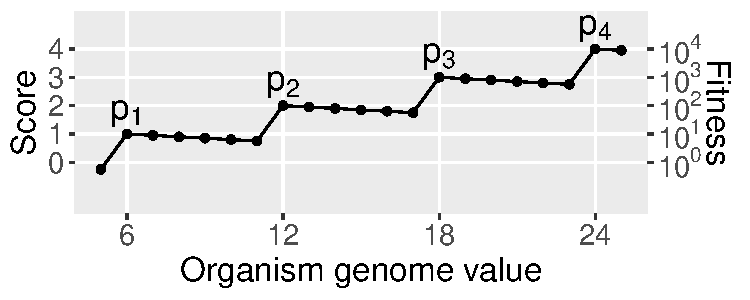
\includegraphics[width=0.75\textwidth]{05_adaptive_momentum/media/sawtooth_conceptual_figure.pdf}
\caption{
    The sawtooth function used in this work, with the four peaks mentioned in this work labeled.
    Score, $s(x)$, and fitness are both shown, with fitness being $10^{s(x)}$.
    %The function and parameters are available in methods. 
}
\label{fig-sawtooth}
\end{center}
\end{figure}

We evolved populations of 512 organisms in a one-dimensional spatial population -- a single line of organisms -- that did not wrap. 
This structure maximizes fixation times and makes selective sweeps easy to track, as they could only move left or right.
The population evolved via discrete, non-overlapping generations. 
%Each new generation of organisms was determined using spatial roulette (i.e., fitness-proportional) selection.%, where roulette selection was performed between the organism and its neighbors (for a maximum of three organisms per selection event). 
To fill positions in the next generation, we performed rounds of spatial roulette selection, each involving three organisms: the organism in that position in the previous generation and its two immediate neighbors (unless the organism is on the edge, in which case the roulette is between only two organisms). 
We then copied the selected individual to produce the offspring, with a $0.0125$ chance to mutate; mutations either increment or decrement the offspring's genome value by one. 
Selective sweeps are thus limited to advancing one position in the population per generation, limiting the growth rate and therefore the fixation time of a beneficial mutation. 
%When an organism is mutated, its integer value is incremented or decremented by one, and we used a mutation of rate of 0.0125 per reproduction event. 

\subsection{Experiment design}

We conducted this work in three stages: 
1) we validated that our model demonstrates adaptive momentum; 
2) we ran ``benchmarking'' data to create an expectation of how potentiation changes during a momentum window; 
and 3) we conducted analytic replay experiments to observe changes in potentiation in evolved lineages. 
Here we outline these experiments in more detail. 

\subsubsection{Experiment I: Model Validation}

%First, we wanted to ensure that our model allowed for valley crossing events, but for those events to be incredibly rare on their own. 
%To accomplish this, we ran 500,000 evolutionary replicates, where each replicate started with 512 organisms at $p_{2}$. 
%These replicates ran for 10,000 generations, much longer than the rest of our experiments, and we tracked the number of generations it took for the populations to cross the valley. 
%Some replicates crossed more than one valley, in which case we recorded the time since the previous crossing. 

%Additionally, we wanted to verify that disequilibrium is what drives the adaptive momentum effect. 

%The goal for our initial experiment was 
To ensure that our model could produce the adaptive momentum effect, 
%To do so, 
we replicated the primary experiment from \citep{Bohm2024.04.08.588357} comparing crossing times in populations starting from equilibrium versus those starting during the disequilibrium of a previous selective sweep. %were affected by the equilibrium state of a population.
We ran 500,000 evolutionary replicates, where each replicate started with 512 organisms at $p_{1}$ and ran for 5,000 generations. 
%, much longer than the rest of our experiments. 
%In the replicates where $p_{2}$ was discovered within in the first 5000 generations, we recorded the number of generations it took to discover $p_{2}$. 
In replicates where $p_{2}$ was discovered, we recorded the generation of discovery and extended the run duration for another 5,000 generations beyond the point of discovery. 
If $p_{3}$ was discovered before time ran out, we recorded this time as well. % to determine if and when $p_{3}$ was discovered. %In replicates that also discovered $p_{3}$, we recorded the number of generations between the discovery of $p_{2}$ and $p_{3}$ if that number was not greater than 5000. 
This methodology produced two time distributions: time to first crossing and time between first and second crossing, both capped at 5,000 generations.
%the first crossing time relative to the start time and the second crossing time relative to the first crossing time.

\subsubsection{Experiment II: Benchmarking}

%Adaptive momentum theory posits that organisms along the leading edge of a selective sweep experience reduced selection, and thus we expected valley crosses to be propelled by the leading edge. 
The adaptive momentum framework posits that populations in disequilibrium experience an increased rate of adaptation. % as long as the disequilibrium persists. 
In spatial populations experiencing a selective sweep, the disequilibrium should manifest near the leading edge of the sweep. 
Specifically, adaptive momentum allows deleterious mutations to accumulate within the advantaged subpopulation along the leading edge. 
This temporarily expanded mutant cloud increases genetic exploration, accounting for an observed increase in the rate of adaptation. 

\begin{figure}[h!]
\begin{center}
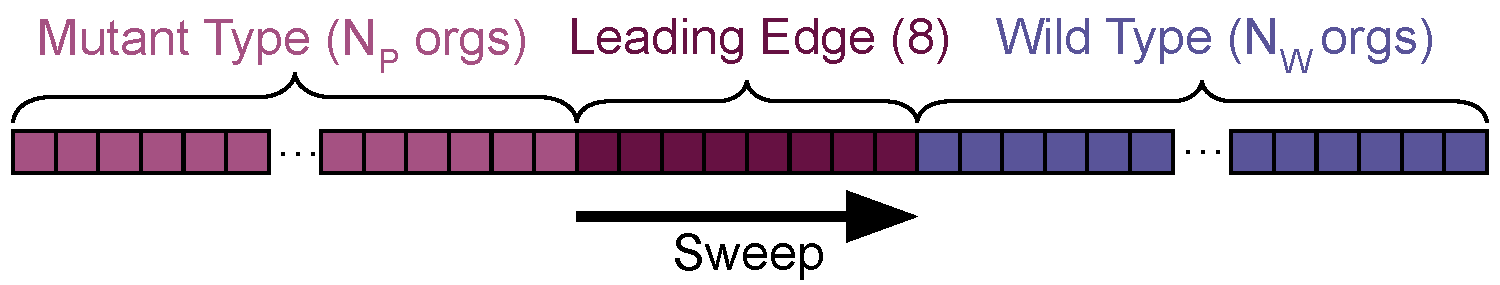
\includegraphics[width=0.85\textwidth]{05_adaptive_momentum/media/sweep_figure.pdf}
\caption{
    Starting layout for experiment II populations, with three clearly-defined sections: $N_P$ ``post-sweep'' mutant organisms at peak $p_{2}$ (left), $N_W$ ``wild type'' organisms at peak $p_{1}$ (right), and 8 ``leading edge'' organisms at a treatment-specific position in the valley past $p_{2}$ (middle).
}
\label{fig-experiment2}
\end{center}
\end{figure}

%We now explain how we apply potentiation to explore these claims.
We created idealized scenarios to study the dynamics of adaptive momentum as they unfold.
Each population had organisms on $p_{2}$ sweeping across organisms on $p_{1}$, with a well-defined leading edge (Fig. \ref{fig-experiment2}).
% of the sweep that are experiencing adaptive momentum.
%  and were experiencing high levels of purifying selection
% and were being swept away
Experimental treatments used all combinations of how far into the next fitness valley the leading edge started (from $x=p_{2}$ to $x=p_{2}+5$), and how far the sweep had progressed across the population (from $N_P=0$, at the beginning of a sweep, to $N_P=504$ at the end.)
%While the leading edge always consisted of eight organisms, its start ranged from position 0 (the beginning of a sweep with no post-sweep organisms) to 504 (the very end of a sweep with no wild-type left), with steps of eight.
%At each position, we tested the six sawtooth values that define a peak and the following valley, from $p_{2}$ to $p_{2} + 5$. 
%The leading edge was always initialized with eight organisms to ensure the post-sweep organisms did not immediately purify the leading edge.
We ran each replicate for $768-N_P$ total generations; the reduced number for larger $N_P$ was used to make the comparison fair, subtracting off the minimum time it could have taken to establish $N_P$ post-sweep organisms.
%, we assumed that if a leading edge is at position $n$ in the population, $n$ updates have already occurred. 
%For example, the replicates with an initial leading edge position of 256 only saw $768 - 256 = 512$ generations of evolution. 
For each condition, we measured how often replicates crossed the next valley to reach $p_{3}$.

We recorded the number of replicates that successfully crossed to $p_{3}$ in each treatment. 
This measurement provided an expectation of a population's potential to cross the valley \textit{based only on the initial state of the leading edge}.
Additionally, we also ran ``shuffled'' controls under otherwise identical conditions, but where we removed population structure (and thus the notion of a leading edge) by randomly shuffling the organisms before each evolutionary replicate.
%The shuffled benchmarks allowed us to evaluate if the population composition was sufficient to account for the results or if the spatial organization of the initialized population, consisting of a leading edge separating the purified post-sweep section from the wild type section, was also important.

\subsubsection{Experiment III: Analytic replays of evolved lineages}

Finally, we focused on the treatment from Experiment II that represented the start of a selective sweep; that is, no post-sweep organisms ($N_P=0$) and a leading edge that just made it to $p_{2}$. %peak 2 ($x=p_{2}$).
We ran 500 replicates under these conditions,
%initialized with the first eight organisms at $p_{2}$ and the rest at $p_{1}$, representing a population at the beginning of a selective sweep shortly after the discovery of a beneficial mutation.
%Again, these replicates evolved for 768 generations. 
saving snapshots at each generation, allowing us to perfectly recreate the population at any time point. 
We randomly selected 10 replicates that failed to reach $p_{3}$, 10 random replicates that did reach $p_{3}$ (but not further), and all four replicates that crossed two valleys to reach $p_{4}$.
For each of these 24 replicates, we performed 1000 analytic replays at every fourth generation, restarting evolution from a given time point with different random seeds to investigate the role of chance in determining \textit{the distribution of potential evolutionary outcomes} \citep{blountContingencyDeterminismEvolution2018}.
Next, we selected one representative sample from each of the three categories to study at high resolution, replaying 10,000 replicates from every generation. 

Using these replays, we recorded the probability that a replicate would cross the valley to $p_{3}$ or $p_{4}$ at each time point. 
These data allow us to calculate how the crossing probabilities changed over time. 
We also ran 10,000 equilibrium replicates and replayed representative replicates in the same manner. 
%This allows us to see how these probabilities changed over time, allowing us to see what generations were key for crossing -- or failing to cross -- that valley. 
%In addition, we recorded the same data for crossing a second valley (to $p_{4}$) in the same manner. 
Finally, just as in the shuffle benchmarking experiment, we performed ``shuffled'' replays on disequilibrium replicates that crossed a single valley.
Specifically, we shuffled the population before starting each replay to measure the role of the population's spatial organization in crossing potential. 

%[TODO - stats?]

\subsection{Data and software availability}
All code, analyses, summarized data, and figures not included in this work are available in the supplemental material \citep{austin_ferguson_2024_11507982}.
The model was built using the Modular Agent Based Evolver version 2.0 (MABE2) (\url{https://github.com/mercere99/MABE2}). 
All analyses and plots were generated using the R statistical computing language version 4.1.2 \citep{r_core_team_r_v4} and the ggplot2 \citep{R-ggplot2}, dplyr \citep{wickhamDplyrGrammarData2022}, HMisc \citep{harrelljrHmiscHarrellMiscellaneous2020}, tidyr \citep{wickhamTidyrTidyMessy2022} packages. %, and khroma \citep{frerebeauKhromaColourSchemes2023} packages. 








% \section{Methods}
% % Here we describe the system used in this paper and detail the experiments conducted. 

% \subsection{Evolution system}
% % We used a minimal agent-based digital evolution model where each organism consists of a single integer genome, where fitness is determined as the expinentiation of the result of a sawtooth function based on genome value ($x$).
% % To calculate fitness we first generate a score using a ``sawtooth'' function, similar to the one used by [CITE preprint], to create a landscape where local optima are separated by deleterious valleys.  
% % Our sawtooth function (\(s\)) is defined as follows: 
% % \[
% % s(x) = kx - (k+d)(x\ \text{mod}\ w)
% % \]

% We used a minimal agent-based evolution model where each organism's genome consists of a single integer, with value $x$. 
% Fitness is based in a repeated ``sawtooth'' function, similar to the one used in \citep{Bohm2024.04.08.588357}, to create a landscape with regular fitness peaks separated by valleys. 
% Each organism is assigned a quality score ($s(x)$), and then that score exponentiated to determine fitness ($f(x)=10^{s(x)}$). Score is calculated using the sawtooth function:

% % \[
% % s(x) = \frac{g}{w}x - (\frac{g}{w}+d)(x\ \text{mod}\ w)
% % \]
% \[
% s(x) = \frac{x - (x~\text{mod}~w)}{w}G - (x~\text{mod}~w)D
% \]

% \noindent
% where $G$ is the gain per peak, $D$ is the decrease per step into the valley, and $w$ is the valley width (number of steps from one peak to the next). 
% Effectively, the score function calculates the quality of the highest peak achieved and subtracts the cost of the current mutational step into the valley. 
% %We used values of \(k = \frac{1}{6}\), \(a = w = 6\), and \(d = 0.05\).
% We used values of $G=1.0$, $D=0.05$, and $w=6$.
% This means that we have peaks appear every six steps; in this case at $x=6$, $x=12$, $x=18$, and so forth.
% We refer to these peaks by their height, so those three peaks would be \(p_{1}\), \(p_{2}\), and \(p_{3}\), respectively.
% We refer to the steps between peaks by the prior peak and an offset (e.g., $x=17$ is $p_{2} + 5$; the last step before $p_{3}$).
% Figure \ref{fig-sawtooth} illustrates this sawtooth function and the relevant peaks.

% Crossing a valley increases an organism's fitness by a factor of 10, and each step into the valley reduces fitness by \localapprox 10\%, regardless of which peak the organism was on.
% We selected these drastic fitness differences to clearly demonstrate the effect rather than be representative of typical biological systems. 
% That being said, while this degree of selective benefit may be rare in biological systems, cases such as antibiotic resistance can show fitness increases of this magnitude \citep{gullbergSelectionResistantBacteria2011}.
% %We stress that the degree of selective advantage modeled here may not represent typical biological systems.

% \begin{figure}[h!]
% \begin{center}
% 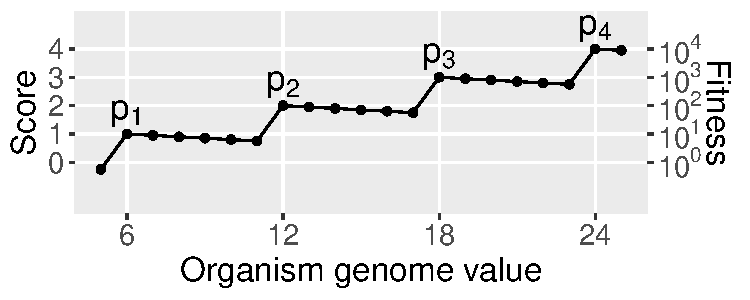
\includegraphics[width=0.75\textwidth]{05_adaptive_momentum/media/sawtooth_conceptual_figure.pdf}
% \caption{
%     The sawtooth function used in this work, with the four peaks mentioned in this work labeled.
%     Score, $s(x)$, and fitness are both shown, with fitness being $10^{s(x)}$.
%     %The function and parameters are available in methods. 
% }
% \label{fig-sawtooth}
% \end{center}
% \end{figure}

% We evolved populations of 512 organisms organized in a one-dimensional spatial population -- a single line of organisms -- that did not wrap. 
% This structure maximizes fixation times and makes selective sweeps easy to track, as they could only move left or right.
% The population evolved via discrete, non-overlapping generations. 
% %Each new generation of organisms was determined using spatial roulette (i.e., fitness-proportional) selection.%, where roulette selection was performed between the organism and its neighbors (for a maximum of three organisms per selection event). 
% To fill a position in the next generation, a round of spatial roulette selection was performed involving three organisms: the organism in that position in the previous generation and its two immediate neighbors (unless the organism is on the edge, in which case the roulette is between only two organisms). 
% The selected individual is then copied to produce an offspring. 
% This copy has a $0.0125$ chance to mutate, which will either increment or decrement the offspring's genome value by one. 
% Selective sweeps are thus limited to advancing one position in the population per generation, limiting the growth rate and therefore the fixation time of a beneficial mutation. 
% %When an organism is mutated, its integer value is incremented or decremented by one, and we used a mutation of rate of 0.0125 per reproduction event. 

% \subsection{Experiment design}

% We conducted this work in three stages: 
% 1) we validated that our model demonstrates adaptive momentum; 
% 2) we ran ``benchmarking'' data to create an expectation of how potentiation changes during a momentum window; 
% and 3) we conducted analytic replay experiments to observe changes in potentiation in the evolved lineages. 
% Here we outline these experiments in more detail. 

% \subsubsection{Experiment I: Model Validation}

% %First, we wanted to ensure that our model allowed for valley crossing events, but for those events to be incredibly rare on their own. 
% %To accomplish this, we ran 500,000 evolutionary replicates, where each replicate started with 512 organisms at $p_{2}$. 
% %These replicates ran for 10,000 generations, much longer than the rest of our experiments, and we tracked the number of generations it took for the populations to cross the valley. 
% %Some replicates crossed more than one valley, in which case we recorded the time since the previous crossing. 

% %Additionally, we wanted to verify that disequilibrium is what drives the adaptive momentum effect. 

% The goal for our initial experiment was to ensure that our model could replicate the adaptive momentum effect. 
% To do so, we replicated the primary experiment from \citep{Bohm2024.04.08.588357} to test whether crossing times were affected by the equilibrium state of a population.
% We ran 500,000 evolutionary replicates, where each replicate started with 512 organisms at $p_{1}$ and ran for 5,000 generations. 
% %, much longer than the rest of our experiments. 
% %In the replicates where $p_{2}$ was discovered within in the first 5000 generations, we recorded the number of generations it took to discover $p_{2}$. 
% In replicates where $p_{2}$ was discovered, we recorded the generation of discovery and extended the run duration for another 5,000 generations beyond the point of discovery. 
% If $p_{3}$ was discovered before time ran out, we recorded this time as well. % to determine if and when $p_{3}$ was discovered. %In replicates that also discovered $p_{3}$, we recorded the number of generations between the discovery of $p_{2}$ and $p_{3}$ if that number was not greater than 5000. 
% This methodology produced two time distributions: time to first crossing and time between first and second crossing, both capped at 5,000 generations.
% %the first crossing time relative to the start time and the second crossing time relative to the first crossing time.

% \subsubsection{Experiment II: Benchmarking}

% %Adaptive momentum theory posits that organisms along the leading edge of a selective sweep experience reduced selection, and thus we expected valley crosses to be propelled by the leading edge. 
% The adaptive momentum framework posits that populations in disequilibrium experience an increased rate of adaptation. % as long as the disequilibrium persists. 
% In spatial populations experiencing a selective sweep, the disequilibrium should manifest near the leading edge of the sweep. 
% Specifically, adaptive momentum allows deleterious mutations to accumulate within the advantaged subpopulation along the leading edge. 
% This temporarily expanded mutant cloud increases genetic exploration, accounting for an observed increase in the rate of adaptation. 

% \begin{figure}[h!]
% \begin{center}
% 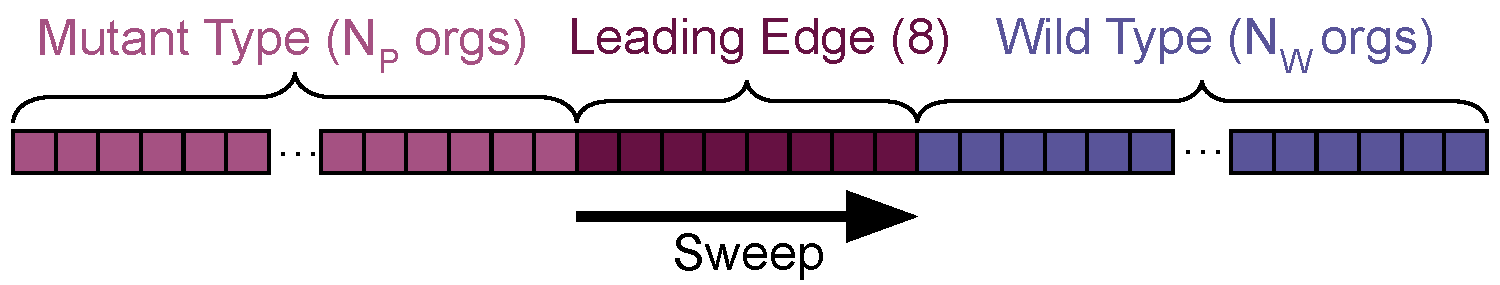
\includegraphics[width=0.85\textwidth]{05_adaptive_momentum/media/sweep_figure.pdf}
% \caption{
%     Starting layout for experiment II populations, with three clearly-defined sections: $N_P$ ``post-sweep'' mutant organisms at peak $p_{2}$ (left), $N_W$ ``wild type'' organisms at peak $p_{1}$ (right), and 8 ``leading edge'' organisms at a treatment-specific position in the valley past $p_{2}$ (middle).
% }
% \label{fig-experiment2}
% \end{center}
% \end{figure}

% %We now explain how we apply potentiation to explore these claims.
% We created idealized scenarios to study the dynamics of adaptive momentum as they unfold.
% Each population had organisms on $p_{2}$ sweeping across organisms on $p_{1}$, with a well-defined leading edge (Fig. \ref{fig-experiment2}).
% % of the sweep that are experiencing adaptive momentum.
% %  and were experiencing high levels of purifying selection
% % and were being swept away
% Experimental treatments used all combinations of how far into the next fitness valley the leading edge started (from $x=p_{2}$ to $x=p_{2}+5$), and how far the sweep had progressed across the population (from $N_P=0$, at the beginning of a sweep, to $N_P=504$ at the end.)
% %While the leading edge always consisted of eight organisms, its start ranged from position 0 (the beginning of a sweep with no post-sweep organisms) to 504 (the very end of a sweep with no wild-type left), with steps of eight.
% %At each position, we tested the six sawtooth values that define a peak and the following valley, from $p_{2}$ to $p_{2} + 5$. 
% %The leading edge was always initialized with eight organisms to ensure the post-sweep organisms did not immediately purify the leading edge.
% We ran each replicate for $768-N_P$ total generations; the reduced number for larger $N_P$ was used to make the comparison fair, subtracting off the minimum time it could take to establish $N_P$ post-sweep organisms.
% %, we assumed that if a leading edge is at position $n$ in the population, $n$ updates have already occurred. 
% %For example, the replicates with an initial leading edge position of 256 only saw $768 - 256 = 512$ generations of evolution. 
% For each condition, we measured how often replicates crossed the next valley to reach $p_{3}$.

% We recorded the number of replicates that successfully crossed to $p_{3}$ in each treatment. 
% This measurement provided an expectation of a population's potential to cross the valley \textit{based only on the initial state of the leading edge}.
% Additionally, we also ran ``shuffled'' controls under otherwise identical conditions, but where we removed population structure (and thus the notion of a leading edge) by randomly shuffling the organisms before each evolutionary replicate.
% %The shuffled benchmarks allowed us to evaluate if the population composition was sufficient to account for the results or if the spatial organization of the initialized population, consisting of a leading edge separating the purified post-sweep section from the wild type section, was also important.

% \subsubsection{Experiment III: Analytic replays of evolved lineages}

% Finally, we focused on the treatment from Experiment II that represented the start of a selective sweep; that is, no post-sweep organisms ($N_P=0$) and a leading edge that just made it to $p_{2}$. %peak 2 ($x=p_{2}$).
% We ran 500 replicates under these conditions,
% %initialized with the first eight organisms at $p_{2}$ and the rest at $p_{1}$, representing a population at the beginning of a selective sweep shortly after the discovery of a beneficial mutation.
% %Again, these replicates evolved for 768 generations. 
% saving snapshots at each generation, allowing us to perfectly recreate the population at any time point. 
% We randomly selected 10 replicates that failed to reach $p_{3}$, 10 random replicates that did reach $p_{3}$ (but not further), and all four replicates that crossed two valleys to reach $p_{4}$.
% For each of these 24 replicates, we performed 1000 analytic replays at every fourth generation, restarting evolution from a given time point with different random seeds to investigate the role of chance in determining \textit{the distribution of potential evolutionary outcomes} \citep{blountContingencyDeterminismEvolution2018}.
% Next, we selected one representative sample from each of the three categories to study at a higher resolution, replaying every generation for 10,000 replicates each. 

% Using these replays, we recorded the probability that a replicate would cross the valley to $p_{3}$ or $p_{4}$ at each of these time points. 
% These data allow us to calculate when and how the crossing probabilities changed over time. 
% We also ran 10,000 equilibrium replicates and replayed representative replicates in the same manner. 
% %This allows us to see how these probabilities changed over time, allowing us to see what generations were key for crossing -- or failing to cross -- that valley. 
% %In addition, we recorded the same data for crossing a second valley (to $p_{4}$) in the same manner. 
% Finally, just as in the shuffle benchmarking experiment, we performed ``shuffled'' replays on disequilibrium replicates that crossed a single valley.
% Specifically, we shuffled the population before starting each replay to determine the role of the population's spatial organization in crossing potential. 

% %[TODO - stats?]

% \subsection{Data and software availability}
% All code, analyses, summarized data, and figures not included in this work are available in the supplemental material \citep{austin_ferguson_2024_11507982}.
% The model was built using the Modular Agent Based Evolver version 2.0 (MABE2) (\url{https://github.com/mercere99/MABE2}). 
% All analyses and plots were generated using the R statistical computing language version 4.1.2 \citep{r_core_team_r_v4} and the ggplot2 \citep{R-ggplot2}, dplyr \citep{wickhamDplyrGrammarData2022}, HMisc \citep{harrelljrHmiscHarrellMiscellaneous2020}, tidyr \citep{wickhamTidyrTidyMessy2022} packages. %, and khroma \citep{frerebeauKhromaColourSchemes2023} packages. 